\documentclass{article}
\usepackage{amsmath}
\usepackage{amssymb}
\usepackage{algorithm}
\usepackage{float}
\usepackage{color}
\usepackage{graphicx}
\graphicspath{ {./} }
\title{Neural Networks Final Project: \\
	\large{Comparing different data pre-processing techniques for convolution neural networks}}
\author{Krystian Wojcicki, 101001444 \\ Michael Kuang, 101000485}
\date{COMP 4107, Fall 2018}

\begin{document}
\maketitle

\newpage

\section{Introduction}

{\em Natural Images} is a dataset currently featured on {\em kaggle.com}. The set is comprised of 6899 images from 8 distinct classes of airplane, car, cat, dog, flower, fruit, motorbike and person. Each class has a varying number of examples. We examined different techniques in pre-processing images and implemented them to analyze their effects on performance in a convolution neural network. 
\section{Background}

One problem we looked at is the Class Imbalance problem, and this is the problem in machine learning where we have great discrepancy in the number of examples between class data. In other words, there are far more examples of one class than another in a set of data. This is a problem because as we know, machine learning works best when we have a more uniform distribution of data. In this project, we examine the performance between two up-sampling techniques called SMOTE and ADASYN as solutions to class imbalance. \\

Another problem we investigated is how image resizing can affect performance. Given a set of non-uniform sizes of images, we must resize them to some constant shape in order to feed examples into the network. We examined two methods; resize the image by scaling it, and crop or pad the image about the center. The problem with resizing an image is that we inevitably lose information as images are scaled down or add noise as they are scaled up. Cropping the image will directly lose the information as we resize the image by cropping out the outer most part of the image, while padding the image with black pixels evenly about center will retain the image aspect ratio.

\section{Problem Statement}
This project attempts to address the problems: "Do different image resizing techniques make a difference to classification accuracy?" and "Do balanced datasets improve classification accuracy?".

\section{Results}

\section{Analysis}

\section{Discussion}

\section{Conclusion	}

\section{References	}

\section{Spatial Pyramid Pooling}

CNNs require a fixed input image size such as 32x32, 64x64 or 128x128 as experimented with in this report. This requirement is human made and artificial while also potentially decreasing recognition accuracy due to loss of content while padding or distortion while resizing. The need to fixed size inputs is due to the fully-connected layer portion of a CNN, the convolution layers use a sliding window and operate correctly on any size input. However the fully-connected portion requires a fixed-size input. To get around this Kaiming et al [2015] introduced spatial pyyramid pooling (SPP), this pooling layer is added on top of the final convolution layer and generates fixed-length outputs regardless of the size of the feature maps given to it.  \\

SPP builds on and improves the concept of Bag-of-Words (BoW), it does so but maintaining spatial information by pooling in local spatial bins. These spatial bins have sizes that are proportional to the image size meaning that the number of bins is fixed regardless of the image size.

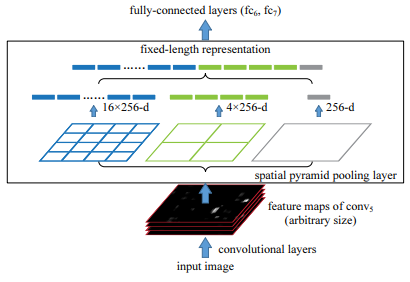
\includegraphics{spp}

For training and testing a model with an SPP layer several approaches can be taken. We chose to investigate a multi-size training approach, here we create two fixed-size networks that share parameters. Then for training we alternated by providing the network 32x32 images for one epoch and then 64x64 epochs for the next epoch. 

\end{document} 